\label{ch:theory}

In this chapter, the fundamental theory, methodology and protocols used in this implementation are introduced. This chapter is intended to provide the reader with an intuitive understanding of the underlying theory, to better understand the design choices. As previously stated, property driven development is the methodology this thesis is based on. Before delving in to PDD it is important to clarify what \textit{Interval Property Checking} (IPC) is and how it can be used to create a sound relationship between ESL and RTL descriptions by means of \textit{Path Predicate Abstraction} (PPA). In Sec.~\ref{sec:ipc} IPC is described together with necessary additional information. What PPA is and how it is used to bridge the semantic gap is covered in Sec.~\ref{sec:ppa}. Sec.~\ref{sec:pdd} then explains PDD and the certain rules it imposes on the ESL descriptions. Finally the AMBA-AHB specification is reviewed in Sec.~\ref{sec:ahb}.       


\section{Interval Property Checking}
\label{sec:ipc}
Formal verification is an approach of functional verification where design specification is formally formulated as a set of properties. A property checker uses mathematical algorithms to prove that the RTL description fulfills the property set. As opposed to simulation based RTL verification, a carefully designed property set guarantees the absence of bugs in the design. Recent industrial languages such as \textit{Interval Language} (ITL) provide an intuitive alternative to formulate such properties using \textit{Linear Temporal Logic} (LTL). \par
An interval property, is a pair of assumptions $A_{t_0}$ and commitments $C_{t_1}$. The assumptions describe the state and inputs of some RTL cluster over a time $t_0$ whereas the commitments describe the state and outputs of the same RTL cluster over time $t_1$. A property checker attempts to prove that when the assumptions hold on the design, the commitments do as well. Here the time variables $t_0$ and $t_1$ represent a a time period relative to an arbitrary time point $t$. The term interval property is interchangeable with operation property. The property structure is illustrated in Fig.
\ref{fig:exop}.  

\begin{figure}[hbt]
\begin{lstlisting}
  property grant_master is
    assume:
       at t: some_state;
       at t: request_signal;
       at t+1: grant_signal;

    prove:
       at t+2: another_state;
       at t+2: not(request_signal);
       at t+2: address_signals;
  end property; 
\end{lstlisting}
\label{fig:exop}
\caption{Example operation property}
\end{figure}

Starting from all possible starting states the property checker searches for an input sequence and a path in the \textit{Finite State Machine} (FSM) where the implication of the $A_{t_0}$, $C_{t_1}$ pair does not hold. The property checker used in this thesis is Onespin 360 DV, or Onespin for short \cite{onespin}. 

\subsection{Complete Interval Property Checking (C-IPC)}
\label{sub:cipc}
A set of properties only guarantee that the design works according to specification if the appropriate termination criterion is used. This criterion was first defined in \cite{bormannbusch}. For a property set to qualify as complete some conditions must be fulfilled. The idea is that, starting from reset there are properties covering every aspect of the I/O behavior and transitions through all important states of the design. The termination criterion hereby referred to as completeness is checked using the property checker Onespin. The design behavior can be guaranteed by a series of tests.
\begin{enumerate}
 \item \textit{Reset test}: It is proven that reset can be applied deterministically and that all outputs and state variables are determined after reset based on listed assumptions.
 \item \textit{Successor test}: Proves that the assumptions of all properties are either inputs or state variables determined by a preceding property. All properties must be properly hooked together, meaning that all assumptions (except inputs) in a property at time $t$ (left hook) is determined by all preceding properties at the same time point (right hook). This ensures there are no gaps between properties where signals are undefined. 
 \item \textit{Determination test}: Proves that all state variables are determined at the right hook in every property, and that all relevant outputs are determined at all times. What a relevant output is in this context is meant by the validity of certain data. In communication data may be invalid unless f.ex a flag is set, the completeness checker can be told to ignore this value otherwise by describing it as \textit{if(flag) then determined(data)}.
 \item \textit{Case split test}: Proves that there is a property covering every transition between important states of the design. In other words there is a property covering every input scenario in every important state. 
\end{enumerate}

A completeness check is not run automatically on the design, rather a completeness description must be manually created. This description contains all inputs, determination requirements (outputs, state variables) and a property graph. It is not generated automatically to help detect faults in the property set rather than having them transferred to the completeness description. As long as only inputs are listed as inputs in the completeness description, and all outputs are listed as determination requirements, the collective hold of all four tests prove completeness. Out of sheer relevance to this thesis key aspects of the process on how to achieve completeness on a design is provided in the following section. 

\subsection{Gap Free Verification}
\label{sub:gfv}
Out of consistency some terms from the previous section are redefined. A state variable is redefined as a \textit{Visible register}. It is a symbolic register that transfers information from the end of one property, to the start of another. It is not necessarily used to determine the state of the system. This is where the term \textit{Conceptual state} comes in. Earlier referred to as important states, conceptual states are abstractions of actual states in the designs FSM. It may directly map to a state in the FSM, parts of one,  contain many or be a collection of visible registers and inputs of a design. The process of creating a property set that proves completeness is divided in four phases. All the specifics of the four phases will not be recounted here, the curious reader is referred to \cite{gapfree}. Rather some implications and key information are highlighted. \par
The process starts with the definition of the \textit{Conceptual State Machine} (CSM) and a set of skeleton properties are made to represent this CSM in the property graph. All visible registers required to correctly represent the assumptions of the properties are added as local determination requirements and determined at right hook in all properties. By making sure all properties only assume inputs and these registers (at correct time point) the successor test will hold. Further, all outputs are listed as determination requirements together with the remaining visible registers needed to help determine them, they are subsequently determined in all properties. If this is done correctly the determination test will hold. Outputs are only determined based on inputs and visible registers. If the mapping of a visible register is incorrect or missing, this is sure to appear as an error in the completeness check. If all possible transitions of the CSM is covered by properties, the case split test will hold. If not, these operations are identified with help of the debugger and added until the case split test holds. The reset test is a special case of these three tests for the reset property, the difference being that it has no predecessor. It is checked alongside the other three tests. When all four tests hold, the property set is complete. 

\subsubsection{Clusters}
\label{sub:clust}
When developing a property set it is sometimes necessary to consider the \textit{Design under Verification} (DuV) as multiple modules communicating with each other. It is not always beneficial to divide the DuV at the RTL module interfaces. The term cluster is therefore introduced to avoid confusion between the two. A design is ideally verified in a single cluster, to keep abstraction at the highest level. In some cases verifying a design in a single cluster is not feasible. The main reason for this is parallelism.\\ 
\begin{wrapfigure}{l}{5.5cm}
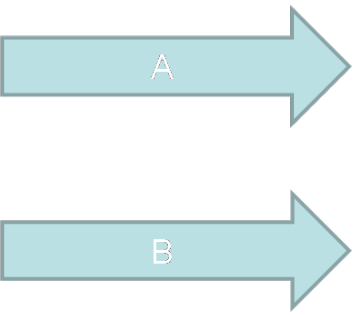
\includegraphics[width=5.5cm]{figs/Verif/parallell.png}
\caption{Parallel data flow}\label{fig:para}
\end{wrapfigure} 

Consider two data flows occurring in parallel. To verify this completely, every scenario must be accounted for. A gets data and not B, B gets data and not A, both A and B or neither. This needs to be accounted for in every clock cycle. In a large design with many operation properties, verification becomes unfeasible even with two parallel data flows.     


Where one draws the conceptual border of a cluster, often falls naturally on the interface between two modules. Sometimes however, it is necessary to do a cluster split where the border consists of arbitrary signals in the middle of a module. Any signal can be determined as an input or output to the completeness plan of a cluster\cite{clust}. When splitting a design into clusters it is important to verify all clusters completely and that any signal that is defined as an input to a cluster is either an input to the design, or an output from another cluster. When defining the signals that represent inputs and outputs between clusters it is recommended to use the same signal names in both clusters. An example of this is using the top level signal in the RTL design that connects cluster A to cluster B. This is to eliminate the possibility that an output from cluster A actually represent a different signal than its respective input to cluster B. By following these guidelines there are no gaps in verification between the clusters. 



\section{Path Predicate Abstraction}
\label{sec:ppa}

This section reviews the principles of PPA and how it is used to abstract the RTL using operation properties. This does not serve as a standalone description of the full theory, for that the reader is referred to \cite{2014-UrdahlStoffel.etal}. To give an understanding of the abstraction mechanism, PPA is discussed with regard to FSM's. \\
Consider an arbitrary RTL design and its accompanying FSM. This FSM has its own input and output alphabet and describes a possibly complex sequence of operations. PPA is used to simplify this sequence of operations by identifying only the important states, a process illustrated with operational graph coloring. \\ 

\begin{figure}[hbt]
\label{fig:ppa}
 \centering
 \begin{subfigure}[b]{0.4\linewidth}
 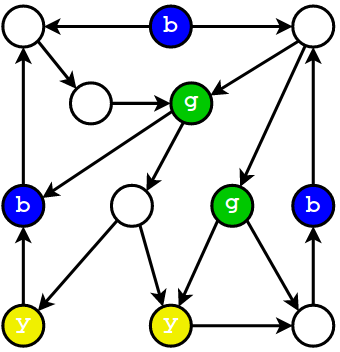
\includegraphics[width=\linewidth]{figs/opcoloring.png}
 \caption{Operationally colored graph}
 \end{subfigure}
 \begin{subfigure}[b]{0.3\linewidth}
 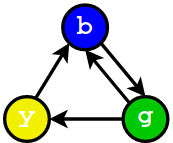
\includegraphics[width=\linewidth]{figs/ppa.png}
 \caption{Resulting PPA}
 \end{subfigure}
\end{figure}

With operational coloring one is able to choose quite freely which states to group together in a conceptual state, and which to leave out as "unimportant" states as long as two rules are followed. 
\begin{enumerate}
 \item All cyclic paths must be broken by at least one colored node, there must be no cyclic path in only uncolored nodes. 
 \item If there is a path between two colored nodes $g\rightarrow y$, there must exist a path to a node of color $y$ from any node of color $g$. 
\end{enumerate} 

Figure \ref{fig:ppa} a) shows the operationally colored FSM of the RTL and b) shows the resulting PPA. It can be easily verified that the color sequence of any path in a) is represented in b). Through abstraction the FSM has been greatly simplified, although some information is lost in the process. It is not possible to extract the original FSM based on the abstraction. An accompanying abstraction of the input and output alphabet of the original must be derived. A communication spanning several nodes in the FSM can now be represented using a single compound in one transition. What before was SDRAM controllers \textit{burst\_read} spanning eight or more cycles can now be represented as a single operation with $sdram\rightarrow read(compound)$. All transitions between the nodes of the PPA together with the abstract input and output alphabet are formulated in operation properties. This set of properties can now be refined to hold on the original design, and a completeness analysis can be run. As covered in section \ref{subsec:cipc} this verifies the complete I/O behavior of the design, and the set of abstract properties can be said to be a sound abstraction of the RTL.  



\section{Property Driven Development}
\label{sec:pdd}
With the PDD methodology a hardware system is represented at the ESL as a product of time-abstract modules communicating at the transaction level. The individual modules of this ESL are analyzed using a software tool \cite{descam} which generates a complete set of operation properties. The modules are designed at the RTL step by step to make the properties hold on the design. When the complete set of properties hold on the design, the ESL is a sound abstraction of the RTL. For a complete overview of the design flow, case studies and proofs the reader is referred to \cite{pddref}. \par
It is not possible to create sound abstractions of hardware modules using arbitrary SystemC constructs. This is particularly true for time abstract SystemC modules. SystemC-PPA defines a subset of SystemC and dedicated communication channels. A module is described in SystemC as an infinite loop iterating over an FSM, where only 32-bit integers, enums and boolean datatypes are allowed. Collections of these datatypes are allowed in structs, so called "compounds". Compounds are used to model communication at the transaction level. Consider a compound containing four data words and addresses. This compound is transferred between two modules in one iteration at the ESL, in contrast to the RTL where it is transferred as a four beat burst. The operation properties are refined such that appropriate address and data words are cycle accurate with respect to the RTL. \par
Communication at the hardware level is divided into two main categories, asynchronous and synchronous. In asynchronous communication transmission is enabled through event signaling, where the receiving end must always be ready to receive such an event. Synchronous communication is enabled through use of a common clock, it is understood through explicit timing that the receiver is ready. There is also the case of unilateral synchronization, where only one communication partner sends such an event. It must then be guaranteed through timing that the other partner is ready. The abstract system model consists of asynchronous PPA's which communicate with each other using events. In SystemC-PPA communication is implemented with channels using port interfaces.


\subsection{Port interfaces}
\label{sub:ports}       
In SystemC-PPA there is three port interfaces available, two of which model the asynchronous and unilateral synchronization mentioned above. The last provide a means of modeling a volatile memory. 

\begin{enumerate}
 \item \textit{Blocking}: The blocking port models asynchronous communication through a four phase handshake. 
 Two modules communicate using $blocking\rightarrow read()$ and $blocking\rightarrow write()$ where the module calling the function is blocked until the other party signals a synchronization signal. 
 This is implemented in SystemC using $event$ and $wait(event)$. This behavior is represented in the properties by use of $notify$ and $sync$ signals for both parties. 
 Each blocking write or read implies an important state and two properties, one for transfer and one for wait. The wait property proves the system is halted; no state, 
 visible registers or outputs are modified while $sync$ is de-asserted. These event notifiers must be implemented in RTL to satisfy both properties, which carries some overhead. 
 To guarantee that no transmission is lost, each notify/sync must be de-asserted in turn between each transfer. There is also a non-blocking alternative available within the interface, 
 which does not guarantee transmission without explicit timing constraints. As a result the system is not halted and a wait property is not generated when using the non-blocking alternative.
  A non-blocking write will however, in any case hand away control by calling a $wait(arbitrary time)$ after every write. The read on the other only calls such a wait if there is no writer blocked on the port.  
 \item \textit{MasterSlave}: To model the unilateral synchronization a master/slave interface models the case where a master can initiate a transfer at any point without regard. The transfer is guaranteed here because the slave will always be ready to respond to the request. The master will issue a synchronization signal and its SystemC-PPA can be modeled rather freely. On the slave side certain rules apply which $DeSCAM$ will check for. All slave ports must be written in every run and no port can be written twice before all other have been and no slave module can use a blocking interface.
 \item \textit{Shared}: The shared port implements no event synchronization and calls no $wait()$ function. It is meant for modeling unordered input data like sensor values. It can be useful to provide additional information in combination with one of the other interfaces.   
\end{enumerate} 

\section{Related work}
\label{sec:related}
The most notable related work is the case study that is the basis of this thesis. 
The case study is concerned with describing a Wishbone bus architecture at the ESL at two different levels of abstraction. 
Both ESL descriptions have interval properties generated, and each their RTL designed based on these properties. 
The case study shows that a higher level of abstraction leads to substantially faster simulation speed. Furthermore, 
the properties from the abstract design are then refined to hold on the less abstract design showing the flexibility of PDD. 
This feature is what this thesis is based on, representing complex multi level hardware using an abstract ESL. The full case study is available in \cite{pddref}.
(need to elaborate, and bring in the ahb formal verification work too)

\section{The AMBA-AHB}
\label{sec:ahb}

This section is a shorthand guide to the AMBA-AHB and its specification to aid in understanding the aspects of the protocol and architecture used in this implementation. For the full AMBA-AHB specification refer to \cite{amba}. The AMBA-AHB is a pipelined high performance bus architecture supporting multiple masters and slaves. Important aspects of the AMBA-AHB are highlighted:

\begin{tabular}{p{3cm} p{10cm}}
Bus master(s) & Can when granted, initiate a transfer, a read or write in the form of a burst or as a single transfer. Multiple master can not transfer concurrently. \\
\hline
Bus slave(s) & Responds to the granted master by reading its control signals in one phase, and responding in the next. \\
\hline
Arbiter & Chooses which master gets a bus grant by using a chosen arbitration scheme. Relevant schemes are fixed priority and round robin. The arbiter controls the address/control and write data mux \\
\hline
Decoder & Decodes the address, selects appropriate slave and controls the response data mux. \\
\hline
Default slave & Response given when no valid slave is selected, it is usually integrated in the decoder.\\
\hline
Default Master & The arbiter grants a selected default master the bus when idle. \\
\end{tabular}


\begin{figure}[hbt]
    \begin{center}
        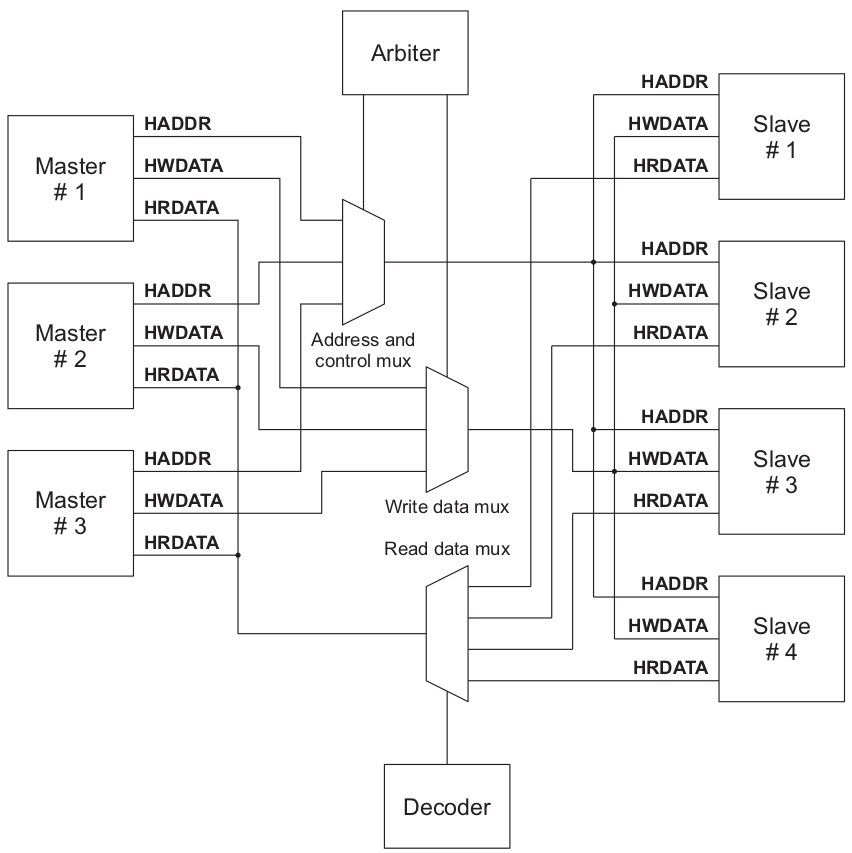
\includegraphics[width=0.8\textwidth]{figs/AHB/AHB_connections.png}
    \end{center}
    \caption{An overview of AHB interconnect, reprinted from \cite{amba}. The mux outputs are referred to as address or data buses.}
    \label{fig:interc}
\end{figure}


\begin{figure}[ht!]
 \centering
 \begin{subfigure}[b]{0.4\linewidth}
 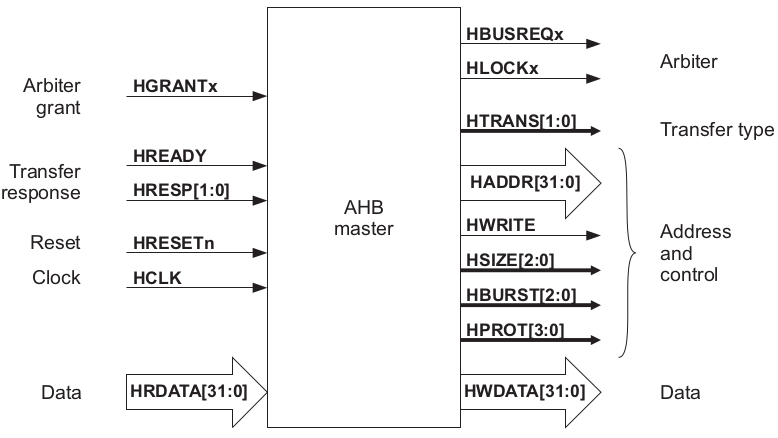
\includegraphics[width=\linewidth]{figs/AHB/master_signals.png}
 \caption{Master signals}
 \end{subfigure}
 \begin{subfigure}[b]{0.4\linewidth}
 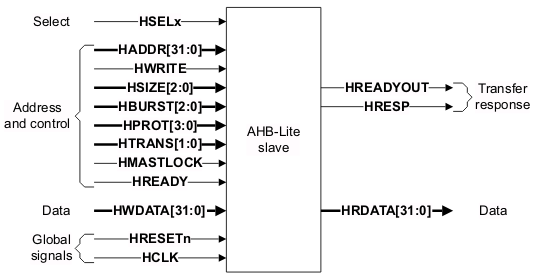
\includegraphics[width=\linewidth]{figs/AHB/slave_lite.png}
 \caption{Slave signals}
 \end{subfigure}
 \caption{Master and slave signals, reprint from a:\cite{amba} b:\cite{amba3}. AHBLite slaves are compatible with AHB systems\cite{ambacomp}. \textbf{HRESP[1:1]} is therefore hardwired to 0.}
 \label{fig:ahbsig}
\end{figure}


As figure \ref{fig:interc} illustrates, the selected address/control and data signals are broadcast to all receivers simultaneously. On the slave side every signal is ignored unless the \textbf{HSELx} signal is set by the decoder. Slave \textbf{x} then reacts to the \textbf{HTRANS[1:0]} and \textbf{HREADY} control signal. \\

\subsection{Overview of transfer}
Before a master can start a transaction it must request access to the bus. The arbiter uses a chosen arbitration method to decide which master is granted access
to the bus. A transaction consists of two phases: \\
\begin{itemize}
 \item Address phase: The master provides address and control signals. The slave must be ready to sample the signals. 
 \item Data phase: Master or slave provides valid data. The slave is able to extend this phase if it is needed. 
\end{itemize}

In the address phase the master provides address and control signals. The control signals tell the slave if it is a read or write, data width and whether the
transfer forms part of a burst. \par
In the data phase data is transferred to or from the slave. If it is a single transfer only one unit of data is transferred. If the slave needs more than
one cycle to process the data it can extend this phase by driving \textbf{HREADY} low. 

\begin{figure}[hbt]
    \begin{center}
        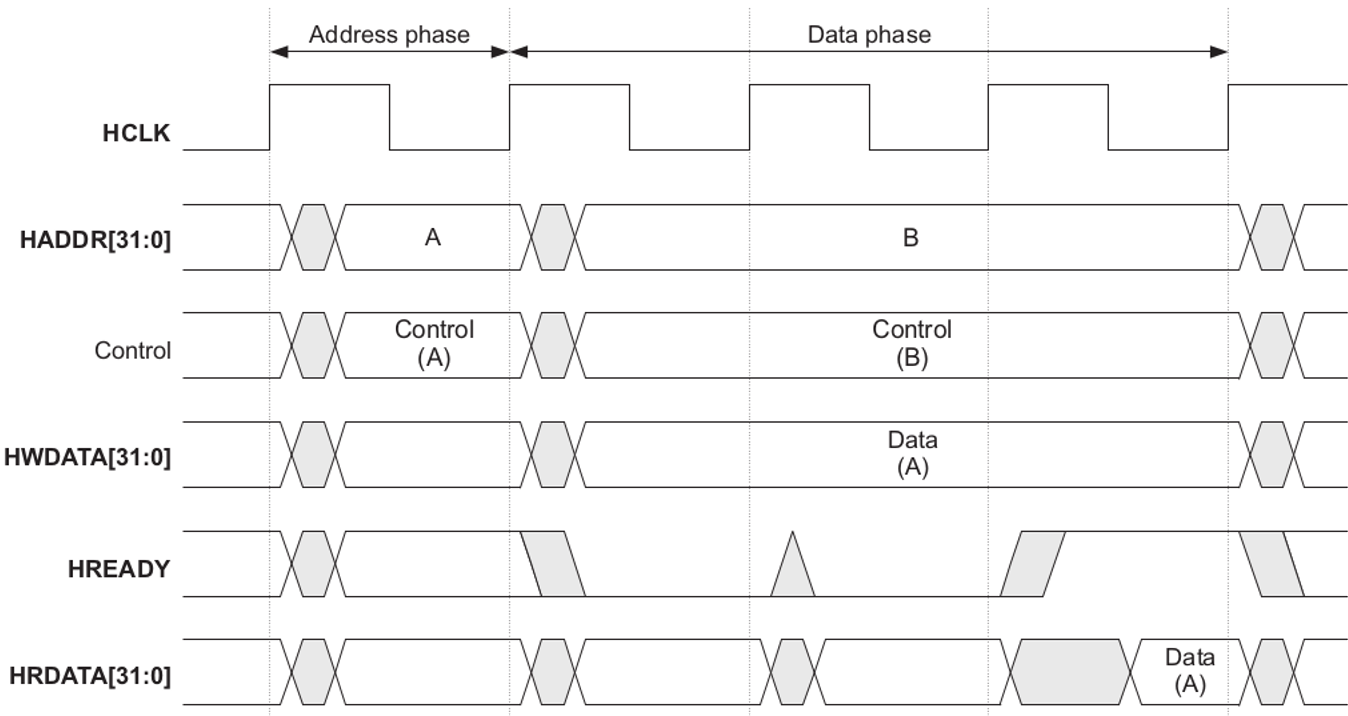
\includegraphics[width=0.8\textwidth]{figs/AHB/transfer.png}
    \end{center}
    \caption{A transfer with wait states, modified reprint from \cite{amba}. In this document the letters represent different masters}
    \label{fig:transfer}
\end{figure}

Figure \ref{fig:transfer} is an example of a transfer that is extended. Observe that in the case of a write transaction, the master must maintain valid \textbf{HWDATA} throughout the entire data phase. In the case of a read, however, the slave must only provide data in the same cycle as it asserts \textbf{HREADY}. Extending the data phase of A has the side effect of extending the address phase of B.  


\newpage
\subsection{Control signals}
The following signals determine which actions the slaves perfom:
\begin{table}[hbt]
  \label{tab:htrans}
  \begin{tabular}{|p{28mm}|r|p{10cm}|} 
  \hline
  \textbf{HTRANS[1:0]} & \textbf{Type} & \textbf{Description} \\
    \hline
  00 & \textit{idle} & No transfer required, used when a master is granted the bus but does not wish to initiate a transfer. Selected slave must always provide a zero wait state \textit{okay} response and ignore all other signals.\\
    \hline
  01 & \textit{busy} & Used by master to insert idle cycles in the middle of a burst sequence. \\
    \hline
  10 & \textit{nonseq} & Indicates the start of a transfer, address and control signals are unrelated to the previous transfer. Single transfers are treated as burst of one, the transfer type is therefore nonsequential\\
    \hline
  11 & \textit{seq} & Address and control signals are related to the previous transfer.\\
\hline
  \end{tabular}
\caption{Transfer type}
\end{table}

\textbf{HWRITE} indicates direction of transfer, a write request is performed when set.

\begin{table}[hbt]
  \label{tab:hsize}
  \begin{tabular}{|p{25mm}|r|p{10cm}|} 
  \hline
  \textbf{HSIZE[2:0]} & \textbf{Size} & \textbf{Description} \\
    \hline
  000 & 8 bits & \textit{Byte}\\
    \hline
  001 & 16 bits & \textit{Halfword} \\
    \hline
  010 & 32 bits & \textit{Word}\\
    \hline
  remainder & >32 bits & \textit{not implemented}.\\
\hline
  \end{tabular}
\caption{Data width}
\end{table}

\subsection{Slave responses}
\label{subsec:slvresp}
After a transfer has been started only the active slave has the ability to end it. The active uses \textbf{HREADY} in combination with \textbf{HRESP} to signal the status of the transfer. The slave can either extend and complete the transfer, or provide a two cycle error response. 

\begin{table}[hbt]
  \label{tab:hsize}
  \begin{tabular}{|r|r|p{10cm}|} 
  \hline
  \textbf{HRESP} & \textbf{HREADY} & \textbf{Description} \\
    \hline
  0 & 0 & Wait state\\
    \hline
  0 & 1 & Transfer complete/Okay response \\
    \hline
  1 & 0 & First cycle of error response\\
    \hline
  1 & 1 & Second cycle of error response \\
\hline
  \end{tabular}
\caption{Slave responses}
\end{table}

If the address provided on the address bus is outside the range of any existing slave the default slave response must be provided. If the encoding on \textbf{HTRANS[1:0]} is \textit{idle} or \textit{busy} default slave must provide a zero cycle okay response. Otherwise the default slave must provide the two cycle error response. 

\subsection{Burst transfers}
With burst transfers several related addresses are accessed either incrementally or by wrapping on an address boundary. The AHB protocol allows for incremental
 and wrapping bursts of four, eight and 16 beats as well as incremental bursts of undefined length. In this section only a four beat incremental burst is covered. The reader is referred to the AMBA specification for the full burst overview \cite{amba}.

\begin{figure}[hbt]
    \begin{center}
        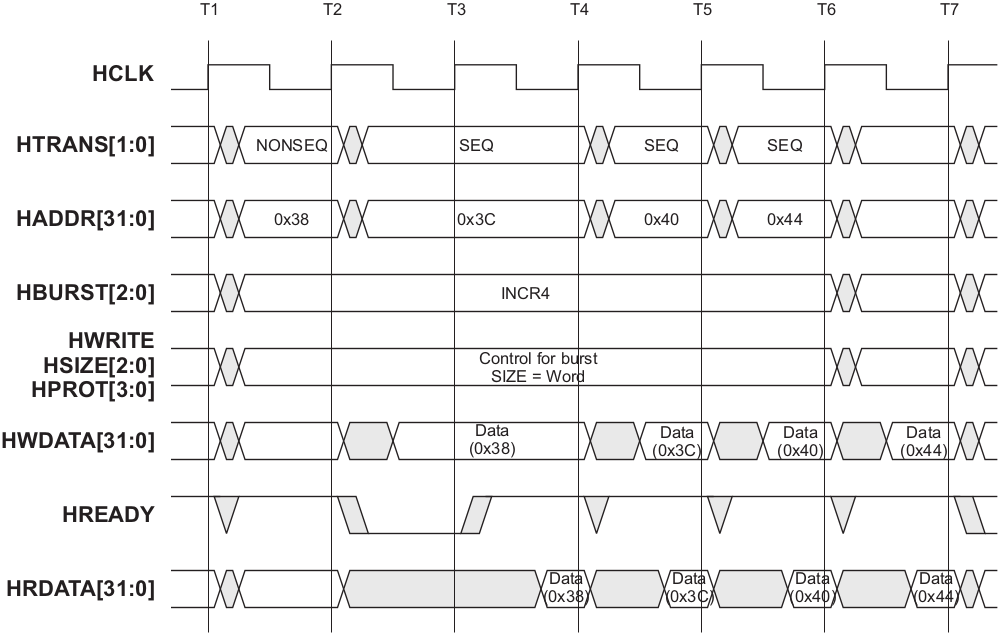
\includegraphics[width=0.8\textwidth]{figs/AHB/burst.png}
    \end{center}
    \caption{A 4 beat incremental burst transfer}
    \label{fig:burst}
\end{figure}

The four beat incremental burst is used to transfer four units of data to or from the selected slave. The address is calculated by incrementing the base address
with amount of bytes encoded on \textbf{HSIZE[2:0]}. Although the address can be calculated using the other fixed control signals, the master must provide the correct address for each beat of the burst. As seen between $T2$ and $T4$ in figure \ref{fig:burst}, wait states can be inserted to bursts as well. \par
There are circumstances where bursts are not allowed to complete because a master loses ownership of the bus. There are however arbitration schemes where this is disabled. If a master receives an error response during a burst it is free to choose whether to complete or abort the transfer. The master must make sure
that an incrementing burst does not cross a 1kB boundary.  



